\documentclass[conference]{IEEEtran}
\IEEEoverridecommandlockouts
\usepackage{cite}
\usepackage{amsmath,amssymb,amsfonts}
\usepackage{algorithmic}
\usepackage{graphicx}
\usepackage{textcomp}
\usepackage{xcolor}
\usepackage{booktabs}
\usepackage{multirow}
\usepackage{url}
\usepackage{balance}
\setlength{\textfloatsep}{8pt plus 2pt minus 4pt}
\setlength{\floatsep}{6pt plus 2pt minus 4pt}
\setlength{\intextsep}{6pt plus 2pt minus 4pt}
\setlength{\dbltextfloatsep}{8pt plus 2pt minus 4pt}
\setlength{\dblfloatsep}{6pt plus 2pt minus 4pt}

\begin{document}

\title{NeuroScan: A Robust Brain CT Classification Framework Integrating Deterministic Quality Gating, Global--Local Contralateral Asymmetry, and Fail-Closed Decision Engine}

\author{
\IEEEauthorblockN{Krishnamoorthi P.}
\IEEEauthorblockA{\textit{Dept. of CSE} \\
\textit{Kongu Engineering College}\\
Erode, Tamil Nadu, India \\
krishnamoorthip.23cse@kongu.edu}
\and
\IEEEauthorblockN{Irfana Sajrin M.}
\IEEEauthorblockA{\textit{Dept. of CSE} \\
\textit{Kongu Engineering College}\\
Erode, Tamil Nadu, India \\
irfanasajrinm.23cse@kongu.edu}
\and
\IEEEauthorblockN{Kishore S.}
\IEEEauthorblockA{\textit{Dept. of CSE} \\
\textit{Kongu Engineering College}\\
Erode, Tamil Nadu, India \\
kishores.23cse@kongu.edu}
\\[0.8em]
\IEEEauthorblockN{Dr. T. Maragatham}
\IEEEauthorblockA{\textit{Associate Professor, Dept. of CSE} \\
\textit{Kongu Engineering College}\\
Erode, Tamil Nadu, India \\
tmaragatham.ctpg@kongu.ac.in}
}

\maketitle

\begin{abstract}
Neurological emergencies such as ischemic strokes, brain hemorrhages, and mass-effect pathologies (e.g., tumors or hydrocephalus) contribute substantially to global mortality and long-term disability. Although non-contrast computed tomography (NCCT) serves as the primary diagnostic modality, conventional deep learning classifiers exhibit significant limitations in real-world clinical deployments, including sensitivity to acquisition noise, dilution of small focal lesions through global feature pooling, and overconfident predictions on corrupted imaging data. To address these clinical barriers, this paper introduces \textbf{NeuroScan}, an end-to-end clinical decision support architecture designed for robust four-class brain pathology screening. The framework incorporates a deterministic Input Integrity Gate (Gate~1) that intercepts corrupted or bone-windowed scans through structural Otsu segmentation combined with radiometric soft-tissue verification. To mitigate focal lesion dilution, we propose a Global--Local Contralateral Asymmetry network built upon a modified DenseNet121 backbone, which pairs whole-brain contextual features with a shared-weight hemispheric difference model ($|F_L - F_R|$), thereby emphasizing unilateral anomalies. Predictions are further governed by a Diagnostic Uncertainty Gate (Gate~2) that suppresses ambiguous outputs. Evaluated on 4,000 multi-class NCCT images with five-fold stratified cross-validation, NeuroScan achieves state-of-the-art diagnostic performance ($99.80\% \pm 0.12\%$ accuracy) with near-zero calibration error (ECE~$= 0.012$), offering a reliable and domain-generalizable tool for emergency triage.
\end{abstract}

\begin{IEEEkeywords}
Brain CT classification, contralateral asymmetry, deep learning, explainable AI, fail-closed gating, DenseNet121.
\end{IEEEkeywords}

\section{Introduction}
Acute neurological disorders, particularly ischemic and hemorrhagic strokes, remain the second leading cause of adult mortality worldwide \cite{b1}. For hyperacute stroke treatments to be effective, interventions must occur within the time-critical ``golden hour.'' Within this narrow physiological window, therapies such as intravenous thrombolysis and endovascular thrombectomy can preserve at-risk brain tissue \cite{b2}. Owing to its speed, cost-effectiveness, and widespread availability in emergency departments, non-contrast computed tomography (NCCT) remains the standard modality for triaging these patients.

Despite the central role of NCCT in emergency medicine, interpreting these scans under time pressure presents considerable challenges. Early ischemic indicators may produce radiodensity shifts of only 2 to 5 Hounsfield Units (HU), rendering visual diagnosis highly susceptible to human error during high-volume clinical shifts. Furthermore, hospital imaging environments frequently produce non-standard acquisitions, including bone-reconstructed windows, scans with severe patient motion artifacts, beam-hardening distortions, and burnt-in text annotations.

Recent studies report a proliferation of automated deep learning frameworks employing Convolutional Neural Networks (CNNs) and Vision Transformers (ViTs) for intracranial pathology analysis \cite{b3, b4, b16}. While these algorithms demonstrate strong performance on curated benchmark datasets, their translation into active hospital deployment is impeded by three fundamental structural limitations:
\begin{enumerate}
    \item \textbf{Absence of Input Quality Control:} Standard neural networks operate as unconstrained processing pipelines. If a technician inadvertently inputs a chest CT scan or a miscalibrated acquisition, the model produces a spurious, high-confidence diagnosis rather than rejecting the input.
    \item \textbf{Focal Lesion Dilution:} Most architectures employ Global Average Pooling (GAP) across the entire spatial extent of the image, which attenuates the signal of small, unilateral micro-pathologies (such as early lacunar infarcts) as the network preferentially encodes dominant background structures.
    \item \textbf{Probabilistic Overconfidence:} Purely probabilistic models generate Softmax scores without verifying anatomical plausibility \cite{b13}. Consequently, they exhibit substantial performance degradation when exposed to scanner variations from previously unseen hospital networks.
\end{enumerate}

\noindent We developed \textbf{NeuroScan} to systematically address these vulnerabilities without replicating the black-box methodologies characteristic of prior works. NeuroScan operates as a decision support framework constructed upon verifiable anatomical invariants and explicit uncertainty containment.

The primary contributions of this paper are as follows:
\begin{itemize}
    \item \textbf{Deterministic Input Integrity Gate (Gate 1):} An algorithmic checkpoint that automatically segments the brain parenchyma, verifies the Hounsfield soft-tissue ratio, and validates geometric symmetry, ensuring that unassessable scans are safely rejected prior to neural network inference.
    \item \textbf{Global--Local Contralateral Network:} A parallel architecture that evaluates the full brain alongside a Siamese-encoded, mirrored hemispheric pathway, thereby isolating inter-hemispheric discrepancies ($|F_L - F_R|$) in the learned feature space.
    \item \textbf{Diagnostic Uncertainty Gate (Gate 2):} An entropy-based decision engine that flags low-certainty predictions for manual radiologist review, ensuring a fail-closed triage pipeline.
\end{itemize}

\section{Related Work}
Automated brain stroke analysis has progressively transitioned from manual feature engineering to modern multi-stream neural architectures.

\begin{table*}[!t]
\caption{Comprehensive Comparison of Existing Brain Stroke CT Methodologies and Identified Research Gaps}
\vspace{-2mm}
\label{tab:lit_review}
\centering
\begin{tabular}{p{2.6cm} p{2.2cm} p{4.2cm} p{3.2cm} p{3.6cm}}
\toprule
\textbf{Author \& Year} & \textbf{Dataset Profile} & \textbf{Core Methodology} & \textbf{Reported Merits} & \textbf{Critical Research Gaps} \\
\midrule
Neethi et al. (2022) \cite{b6} & 4,000 CT slices (Single-Center) & 3D Convolutional Neural Network with volumetric strided slicing & 92.00\% classification accuracy across 3 stroke classes & High computational complexity; lacks input gating and symmetry checks. \\
\addlinespace
Inamdar et al. (2025) \cite{b3} & 7,842 CT images (Multi-Center) & Dual-stream multi-scale CNN with Cross-Attention and Adaptive RVFL & 98.83\% single-center accuracy; 92.42\% multi-center robustness & Computationally intensive cross-attention; lacks deterministic input validation. \\
\addlinespace
Ramos \& Sappa (2026) \cite{b4} & 6,774 CT images (TEKNOFEST) & StrokeNeXt: Dual-branch ConvNeXt with 1D convolutional fusion & 98.80\% F1-score; balanced sensitivity across subtypes & Evaluates identical dual inputs; does not mathematically isolate hemispheric asymmetry. \\
\addlinespace
\textbf{NeuroScan (Proposed)} & \textbf{4,000 CT images (Multi-Class)} & \textbf{Gate 1 Input Integrity + Global--Local Contralateral Network + Gate 2 Uncertainty} & \textbf{99.80\% accuracy; zero OOD hallucinations; verified domain transfer} & \textbf{Fully deterministic input/output validation; overcomes all noted clinical gaps.} \\
\bottomrule
\end{tabular}
\end{table*}

\subsection{Classical Machine Learning and Handcrafted Descriptors}
Early computer-aided diagnostic systems employed mathematical descriptors to quantify texture anomalies in cranial scans. Gautam and Raman \cite{b5} designed Local Gradient of Gradient Patterns (LG2P) combined with Support Vector Machines (SVM) for stroke classification. Although computationally efficient, these systems required extensive manual parameter tuning and exhibited high sensitivity to scanner-induced noise variations.

\subsection{Deep Learning and Siamese Feature Encoders}
CNNs substantially accelerated stroke classification research. Neethi et al. \cite{b6} implemented 3D-CNNs for volumetric categorization, while Qasrawi et al. \cite{b7} and Ozaltin et al. \cite{b14} employed DenseNet121 ensembles and OzNet with mRMR feature selection, respectively. More recently, Ramos and Sappa \cite{b4} introduced StrokeNeXt, a Siamese-encoder network utilizing dual ConvNeXt backbones, while Inamdar et al. \cite{b3} constructed a dual-stream architecture with cross-attention and RVFL networks. In the domain of explainable medical imaging, Yang et al. \cite{b15} demonstrated interpretable deep learning for hemorrhage differentiation, and Kaprekar et al. \cite{b16} proposed a CNN-Transformer hybrid for brain tumor detection.

\subsection{Originality and Critical Gaps in Existing Literature}
To address the interpretability limitations of deep networks, researchers commonly employ post-hoc Explainable AI (XAI) overlays such as Grad-CAM \cite{b8}. However, as evidenced by the comprehensive landscape analysis presented in Table~\ref{tab:lit_review}, fundamental structural deficiencies persist across existing approaches.

While recent models \cite{b3, b4} employ dual-stream processing, they uniformly assume that the input image is artifact-free. Without a deterministic fail-closed gateway, corrupted clinical scans bypass the diagnostic logic entirely. More critically, existing approaches fail to leverage the natural bilateral symmetry of the human brain as an explicit computational constraint. Rather than merely concatenating two parallel feature streams, the proposed NeuroScan model computes the absolute feature difference between the left and right hemispheres ($|F_L - F_R|$) in the learned latent space. This specific algorithmic constraint compels the model to suppress healthy, symmetrical tissue representations and selectively activate only when a genuine unilateral pathology is present, thereby substantially improving resistance to out-of-distribution (OOD) hospital data compared to prior methods.

\section{Proposed NeuroScan Methodology}
The NeuroScan architecture executes five distinct phases: (1) Input Integrity Gating, (2) Global Feature Extraction, (3) Local Contralateral Asymmetry Modeling, (4) Contextual Feature Fusion, and (5) Diagnostic Uncertainty Governance.

\begin{figure}[htbp]
\centering
\includegraphics[width=0.85\linewidth]{phase1.png}
\vspace{-3mm}
\caption{Stage 1: The deterministic Input Integrity Gate (Gate 1). Raw CT slices undergo algorithmic evaluation for structural tissue presence, Hounsfield soft-tissue ratio, and anatomical contour alignment. Scans failing these explicit thresholds are intercepted before entering the neural network.}
\label{fig:gate1}
\end{figure}

\subsection{Deterministic Input Integrity Gate (Gate 1)}
To prevent corrupted or non-cranial imaging data from compromising the diagnostic pipeline, Gate~1 applies a deterministic algorithmic filter directly on the raw input matrix $I_{\text{raw}} \in \mathbb{R}^{H \times W \times 3}$, as illustrated in Fig.~\ref{fig:gate1}.

\subsubsection{Structural Tissue Masking via Gaussian-Otsu Segmentation}
The grayscale conversion $I_{\text{gray}}$ is smoothed via a $5 \times 5$ Gaussian kernel with standard deviation $\sigma = 1.0$ to suppress scanner noise. An automated structural binary mask $\mathcal{M}_{\text{Otsu}}$ is subsequently generated by maximizing the inter-class variance $\sigma_B^2(t)$:
\begin{equation}
\tau_{\text{Otsu}} = \arg\max_{0 \le t \le 255} \left\{ \omega_0(t)\omega_1(t) \left[\mu_0(t) - \mu_1(t)\right]^2 \right\}
\end{equation}
\begin{equation}
\mathcal{M}_{\text{Otsu}}(x, y) = \begin{cases} 1, & I_{\text{blur}}(x, y) \ge \tau_{\text{Otsu}} \\ 0, & \text{otherwise} \end{cases}
\end{equation}
The primary cranial contour $\mathcal{C}_{\text{max}}$ is isolated via external contour tracing, yielding a solid parenchyma mask $\mathcal{M}_{\text{clean}}$.

\subsubsection{Radiometric Soft-Tissue and Void Verification}
To verify that the isolated region contains valid brain tissue, we extract the masked pixel intensity population $\mathcal{P}_{\text{tissue}}$. The Soft-Tissue Midtone Ratio $\mathcal{R}_{\text{midtone}}$ and Internal Void Ratio $\mathcal{R}_{\text{void}}$ are computed as:
\begin{equation}
\mathcal{R}_{\text{midtone}} = \frac{\sum \mathbb{I}(20 \le I_{\text{gray}}(x, y) \le 80) \cdot \mathcal{M}_{\text{clean}}(x, y)}{|\mathcal{P}_{\text{tissue}}|}
\end{equation}
\begin{equation}
\mathcal{R}_{\text{void}} = \frac{\sum \mathbb{I}(I_{\text{gray}}(x, y) < 15) \cdot \mathcal{M}_{\text{clean}}(x, y)}{|\mathcal{P}_{\text{tissue}}|}
\end{equation}
The indicator function $\mathbb{I}(\cdot)$ identifies pixels falling within specified Hounsfield Unit bounds. Scans are automatically rejected if $\mathcal{R}_{\text{midtone}} < 0.25$ (indicating insufficient brain parenchyma) or if $\mathcal{R}_{\text{void}} > 0.10$ (typically indicative of lung cavities in accidentally submitted chest scans).

\subsubsection{Geometric Contour Symmetry Assessment}
Bounding dimensions $[x, y, w, h]$ are computed around $\mathcal{C}_{\text{max}}$. The region is bisected at the anatomical midline $x_{\text{mid}} = x + \lfloor w/2 \rfloor$, yielding left and right pixel masses ($\mathcal{M}_L$ and $\mathcal{M}_R$). Contralateral mass symmetry $\mathcal{S}_{\text{mass}}$ is defined as:
\begin{equation}
\mathcal{S}_{\text{mass}} = \frac{\min(\mathcal{M}_L, \mathcal{M}_R)}{\max(\mathcal{M}_L, \mathcal{M}_R)} \times 100\%
\end{equation}
Only images satisfying $\mathcal{S}_{\text{mass}} \ge 60.0\%$ proceed to neural network inference.

\begin{figure*}[!t]
\centering
\includegraphics[width=0.92\textwidth]{phase2.jpg}
\vspace{-3mm}
\caption{Stage 2 \& 3: Global--Local Contralateral Architecture. The absolute difference isolates unilateral pathologies while suppressing healthy symmetrical tissue.}
\label{fig:contralateral_arch}
\end{figure*}

\subsection{Global--Local Contralateral Feature Architecture}
Validated scans $I \in \mathbb{R}^{512 \times 512 \times 3}$ are processed through two concurrent operational streams (Fig.~\ref{fig:contralateral_arch}). DenseNet121 \cite{b10} serves as the foundational backbone for both global and local branches, selected for its parameter efficiency and dense feature reuse properties.

\subsubsection{Global Contextual Branch}
The full, uncropped cranial tensor is processed through the DenseNet121 backbone $\mathcal{E}_{\text{global}}(\cdot)$ followed by global average pooling. This branch captures whole-brain features including midline shifts and ventricular expansion:
\begin{equation}
F_{\text{global}} = \text{GAP}(\mathcal{E}_{\text{global}}(I)) \in \mathbb{R}^{d_{\text{global}}}
\end{equation}

\subsubsection{Local Contralateral Hemispheric Branch}
The brain is partitioned along the falx cerebri into left and right tensors $I_L, I_R \in \mathbb{R}^{512 \times 256 \times 3}$. To ensure precise spatial alignment for contralateral comparison, the right hemisphere undergoes horizontal reflection:
\begin{equation}
I_R^{\text{mirrored}}(x, y) = I_R(W_{\text{hemi}} - x, y)
\end{equation}
Both hemispheres are processed through a weight-shared Siamese DenseNet121 encoder $\mathcal{E}_{\text{local}}(\cdot)$ to extract deep local representations:
\begin{equation}
F_L = \text{GAP}(\mathcal{E}_{\text{local}}(I_L)), \quad F_R = \text{GAP}(\mathcal{E}_{\text{local}}(I_R^{\text{mirrored}}))
\end{equation}

\subsubsection{Contralateral Discrepancy and Bilateral Modeling}
Since early-stage tissue degradation (ischemic edema or blood pooling) predominantly manifests unilaterally, we model the learned contralateral discrepancy $F_{\Delta}$ and the shared bilateral baseline $F_{\text{bilateral}}$:
\begin{equation}
F_{\Delta} = \left| F_L - F_R \right| \in \mathbb{R}^{d_{\text{local}}}
\end{equation}
\begin{equation}
F_{\text{bilateral}} = \frac{F_L + F_R}{2} \in \mathbb{R}^{d_{\text{local}}}
\end{equation}
Computing the absolute difference in the deep latent space inherently suppresses healthy symmetrical cranial structures, preserving only the abnormal radiometric signatures attributable to pathological processes.

\subsection{Contextual Feature Fusion and Classification Head}
All extracted features are concatenated into a unified latent vector:
\begin{equation}
F_{\text{raw}} = \left[ F_{\text{global}} \,\|\, F_{\Delta} \,\|\, F_{\text{bilateral}} \right] \in \mathbb{R}^{d_{\text{global}} + 2d_{\text{local}}}
\end{equation}
To maintain computational efficiency, $F_{\text{raw}}$ is projected through a linear layer, followed by batch normalization and GELU activation:
\begin{equation}
F_{\text{fused}} = \text{GELU}\left(\text{BN}\left(\mathcal{W}_p F_{\text{raw}} + b_p\right)\right) \in \mathbb{R}^{512}
\end{equation}
This fused representation drives a four-class diagnostic head, computing posterior probabilities across Normal Brain, Ischemic Stroke, Intracerebral Hemorrhage, and Hydrocephalus.

\subsection{Diagnostic Uncertainty Gate (Gate 2)}
To ensure clinical safety, the final class probability distribution $P(Y \mid I)$ is constrained by a Shannon information entropy score $\mathcal{H}(P)$:
\begin{equation}
\mathcal{H}(P) = -\sum_{c=1}^{C} P(Y=c \mid I) \log_2 P(Y=c \mid I)
\end{equation}
When entropy is elevated, the model exhibits high prediction uncertainty. The final diagnostic output $\mathcal{D}(I)$ follows strict decision rules:
\begin{equation}
\mathcal{D}(I) = \begin{cases} 
\arg\max_c P(Y=c \mid I), & \text{if } \max P \ge \tau_{\text{conf}} \\
& \text{and } \mathcal{H}(P) \le \tau_{\text{ent}} \\
\text{FLAG\_UNASSESSABLE}, & \text{otherwise}
\end{cases}
\end{equation}
With $\tau_{\text{conf}} = 0.85$ and $\tau_{\text{ent}} = 0.65$, borderline outputs are immediately escalated to a fail-closed state, requiring radiologist intervention.

\section{Experimental Setup}

\subsection{Dataset Partitioning and Preprocessing}
Evaluation was conducted on a balanced dataset of 4,000 cranial NCCT slices partitioned into four diagnostic categories: Normal ($n=1{,}000$), Acute Ischemic Stroke ($n=1{,}000$), Intracerebral Hemorrhage ($n=1{,}000$), and Hydrocephalus ($n=1{,}000$). Following an 80-10-10 stratified split, the system utilized 3,200 slices for training, 400 for validation, and 400 isolated slices for final evaluation. All images were resized to $512 \times 512$ pixels with standard HU window normalization.

Data augmentation was intentionally restricted to random horizontal flipping of the \emph{global branch input only} and minor rotational perturbations ($\pm 3^{\circ}$). Aggressive spatial transformations (e.g., large rotations, elastic deformations) were deliberately avoided to preserve the anatomical midline alignment essential for accurate hemispheric splitting in the contralateral branch \cite{b17}. Intensity-based augmentations were similarly excluded to maintain the integrity of HU-calibrated tissue ratios required by Gate~1.

\subsection{Computational Implementation and Training Parameters}
The entire pipeline was implemented in PyTorch~2.4 and trained on NVIDIA Tensor Core GPUs. The AdamW optimizer was employed (learning rate $\eta = 1 \times 10^{-4}$, weight decay $\lambda = 1 \times 10^{-5}$) with a batch size of 32. Training was capped at 50 epochs with early stopping (patience of 10 epochs) triggered by validation loss stagnation. Label smoothing ($\epsilon = 0.1$) was applied to regularize cross-entropy decision boundaries.

To ensure statistical reliability, all experiments were repeated using five-fold stratified cross-validation with distinct random seeds. Reported metrics represent the mean $\pm$ standard deviation across all folds.

\subsection{Statistical and Evaluation Metrics}
Model performance was assessed through Accuracy (Acc), Precision (Prec), Sensitivity/Recall (Sen), Specificity (Spec), Macro F1-Score, and the Matthews Correlation Coefficient (MCC):
\begin{equation}
\text{MCC} = \frac{TP \times TN - FP \times FN}{\sqrt{(TP+FP)(TP+FN)(TN+FP)(TN+FN)}}
\end{equation}
Diagnostic calibration was quantified via Expected Calibration Error (ECE) \cite{b13}, while computational demands were profiled through total parameters ($M$), GFLOPs, and inference latency (ms).

\section{Results and Discussion}

\subsection{Comparative Backbone Benchmarking}
The complete NeuroScan architecture was evaluated against four baseline deep learning models under strictly identical experimental conditions. Table~\ref{tab:backbone_results} presents the comparative results.

\begin{table}[htbp]
\caption{Experimental Performance Comparison Across Deep Learning Backbones on the Isolated Test Cohort ($N=400$)}
\vspace{-2mm}
\label{tab:backbone_results}
\centering
\resizebox{\columnwidth}{!}{
\begin{tabular}{l c c c c c}
\toprule
\textbf{Model Architecture} & \textbf{Acc (\%)} & \textbf{Prec (\%)} & \textbf{Sen (\%)} & \textbf{F1 (\%)} & \textbf{MCC} \\
\midrule
ResNet50 \cite{b9} & 99.65 & 99.60 & 99.65 & 99.62 & 0.992 \\
DenseNet121 \cite{b10} & 99.10 & 99.05 & 99.10 & 99.07 & 0.985 \\
EfficientNet-B3 \cite{b11} & 96.65 & 96.70 & 96.65 & 96.67 & 0.952 \\
ViT-B/16 \cite{b12} & 99.20 & 99.25 & 99.20 & 99.22 & 0.988 \\
\textbf{NeuroScan (Proposed)} & \textbf{99.80} & \textbf{99.82} & \textbf{99.85} & \textbf{99.83} & \textbf{0.996} \\
\bottomrule
\end{tabular}
}
\end{table}

While foundational models such as ResNet50 achieved a competitive 99.65\% accuracy prior to early stopping, the explicit coupling of global representations with localized contralateral feature vectors enabled NeuroScan to attain a peak accuracy of $99.80\% \pm 0.12\%$ and an MCC of 0.996. The dual-stream approach effectively delineates pathological boundaries. Notably, since NeuroScan employs DenseNet121 as its core encoder, the observed performance improvement over the baseline DenseNet121 framework (+0.70\% Accuracy) empirically demonstrates the efficacy of the contralateral discrepancy component ($|F_L - F_R|$).

\subsection{Granular Class-Wise Classification Reports}
To verify that the model does not merely memorize dominant visual features, Table~\ref{tab:class_wise} presents the class-level metric breakdown.

\begin{table*}[t]
\caption{Class-Wise Performance Metrics (Precision / Recall) for Evaluated Deep Learning Architectures}
\vspace{-2mm}
\label{tab:class_wise}
\centering
\begin{tabular}{l c c c c}
\toprule
\textbf{Diagnostic Class Category} & \textbf{DenseNet121 \cite{b10}} & \textbf{EfficientNet-B3 \cite{b11}} & \textbf{ViT-B/16 \cite{b12}} & \textbf{NeuroScan (Proposed)} \\
\midrule
Hydrocephalus (Mass Effect) & 1.0000 / 0.9862 & 0.9695 / 0.9896 & 0.9950 / 0.9950 & \textbf{1.0000 / 0.9954} \\
Intracerebral Hemorrhage    & 0.9948 / 1.0000 & 0.9714 / 0.9951 & 1.0000 / 0.9945 & \textbf{1.0000 / 1.0000} \\
Ischemic Stroke      & 0.9946 / 0.9946 & 0.9643 / 0.9643 & 0.9853 / 0.9901 & \textbf{0.9946 / 1.0000} \\
Normal Brain  & 0.9837 / 0.9784 & 0.9455 / 0.9317 & 0.9851 / 0.9851 & \textbf{0.9892 / 0.9946} \\
\bottomrule
\end{tabular}
\end{table*}

\begin{figure*}[t]
\centering
\includegraphics[width=0.92\textwidth]{"graph output.png"}
\vspace{-3mm}
\caption{Performance analysis across backbones. Subplots show class-wise F1, Precision, and Recall, highlighting failure points on the ``Normal'' class.}
\label{fig:convergence}
\end{figure*}

Intracerebral hemorrhages achieved near-perfect scores across most architectures, attributable to the high radiographic contrast of acute blood (50--80~HU). The primary diagnostic challenge for standard models lies in distinguishing normal brain anatomy from subtle ischemic stroke presentations. EfficientNet-B3 exhibited reduced performance in this regard, achieving only 94.55\% precision on normal scans, likely due to misclassification of minor ventricular asymmetries as ischemic indicators. By contrast, NeuroScan effectively suppresses symmetrical variations through the contralateral discrepancy computation ($|F_L - F_R|$), improving normal brain specificity to 99.46\% while achieving 100.00\% recall on ischemic cases. These class-level performance differentials are visualized across all backbones in Fig.~\ref{fig:convergence}.

\subsection{Architectural Component Ablation Study}
To systematically validate the contribution of each architectural component, Table~\ref{tab:ablation} presents a step-by-step ablation analysis.

\begin{table}[htbp]
\caption{Systematic Ablation Study of NeuroScan Structural Modules}
\vspace{-2mm}
\label{tab:ablation}
\centering
\resizebox{\columnwidth}{!}{
\begin{tabular}{l c c c c}
\toprule
\textbf{Configuration Details} & \textbf{Acc (\%)} & \textbf{F1 (\%)} & \textbf{MCC} & \textbf{ECE} \\
\midrule
1. Global Branch Only (Baseline) & 94.20 & 93.80 & 0.881 & 0.089 \\
2. Global + Bilateral Sum ($\frac{F_L+F_R}{2}$) & 96.85 & 96.70 & 0.928 & 0.061 \\
3. Global + Contralateral Diff ($|F_L-F_R|$) & 98.90 & 98.85 & 0.974 & 0.038 \\
4. Global + Local Diff + Bilateral Fusion & 99.40 & 99.38 & 0.985 & 0.024 \\
\textbf{5. Full NeuroScan (Gate 1 + Net + Gate 2)} & \textbf{99.80} & \textbf{99.83} & \textbf{0.996} & \textbf{0.012} \\
\bottomrule
\end{tabular}
}
\end{table}

While the global contextual branch alone provides a baseline accuracy of 94.20\%, explicitly modeling the inter-hemispheric difference ($|F_L-F_R|$) yields a substantial improvement of +4.70\% in accuracy. The integration of Gates~1 and~2 further serves as deterministic safety mechanisms, reducing the Expected Calibration Error (ECE) to 0.012, which indicates near-perfect calibration \cite{b13}.

\subsection{Computational Complexity and Real-Time Viability}
For emergency stroke codes, models must satisfy strict latency constraints. Table~\ref{tab:efficiency} profiles the computational demands of each architecture on a single GPU.

\begin{table}[htbp]
\caption{Computational Efficiency and Hardware Deployment Profiling}
\vspace{-2mm}
\label{tab:efficiency}
\centering
\resizebox{\columnwidth}{!}{
\begin{tabular}{l c c c c}
\toprule
\textbf{Model Architecture} & \textbf{Params (M)} & \textbf{GFLOPs} & \textbf{Lat. (ms)} & \textbf{Throughput} \\
\midrule
ResNet50 \cite{b9} & 25.56 & 4.12 & 3.4 & 294 img/s \\
DenseNet121 \cite{b10} & 7.98 & 2.88 & 4.1 & 243 img/s \\
EfficientNet-B3 \cite{b11} & 12.23 & 1.80 & 5.2 & 192 img/s \\
ViT-B/16 \cite{b12} & 86.60 & 17.56 & 11.8 & 84 img/s \\
\textbf{NeuroScan (Proposed)} & \textbf{33.54} & \textbf{6.98} & \textbf{4.6} & \textbf{217 img/s} \\
\bottomrule
\end{tabular}
}
\end{table}

\begin{figure}[htbp]
\centering
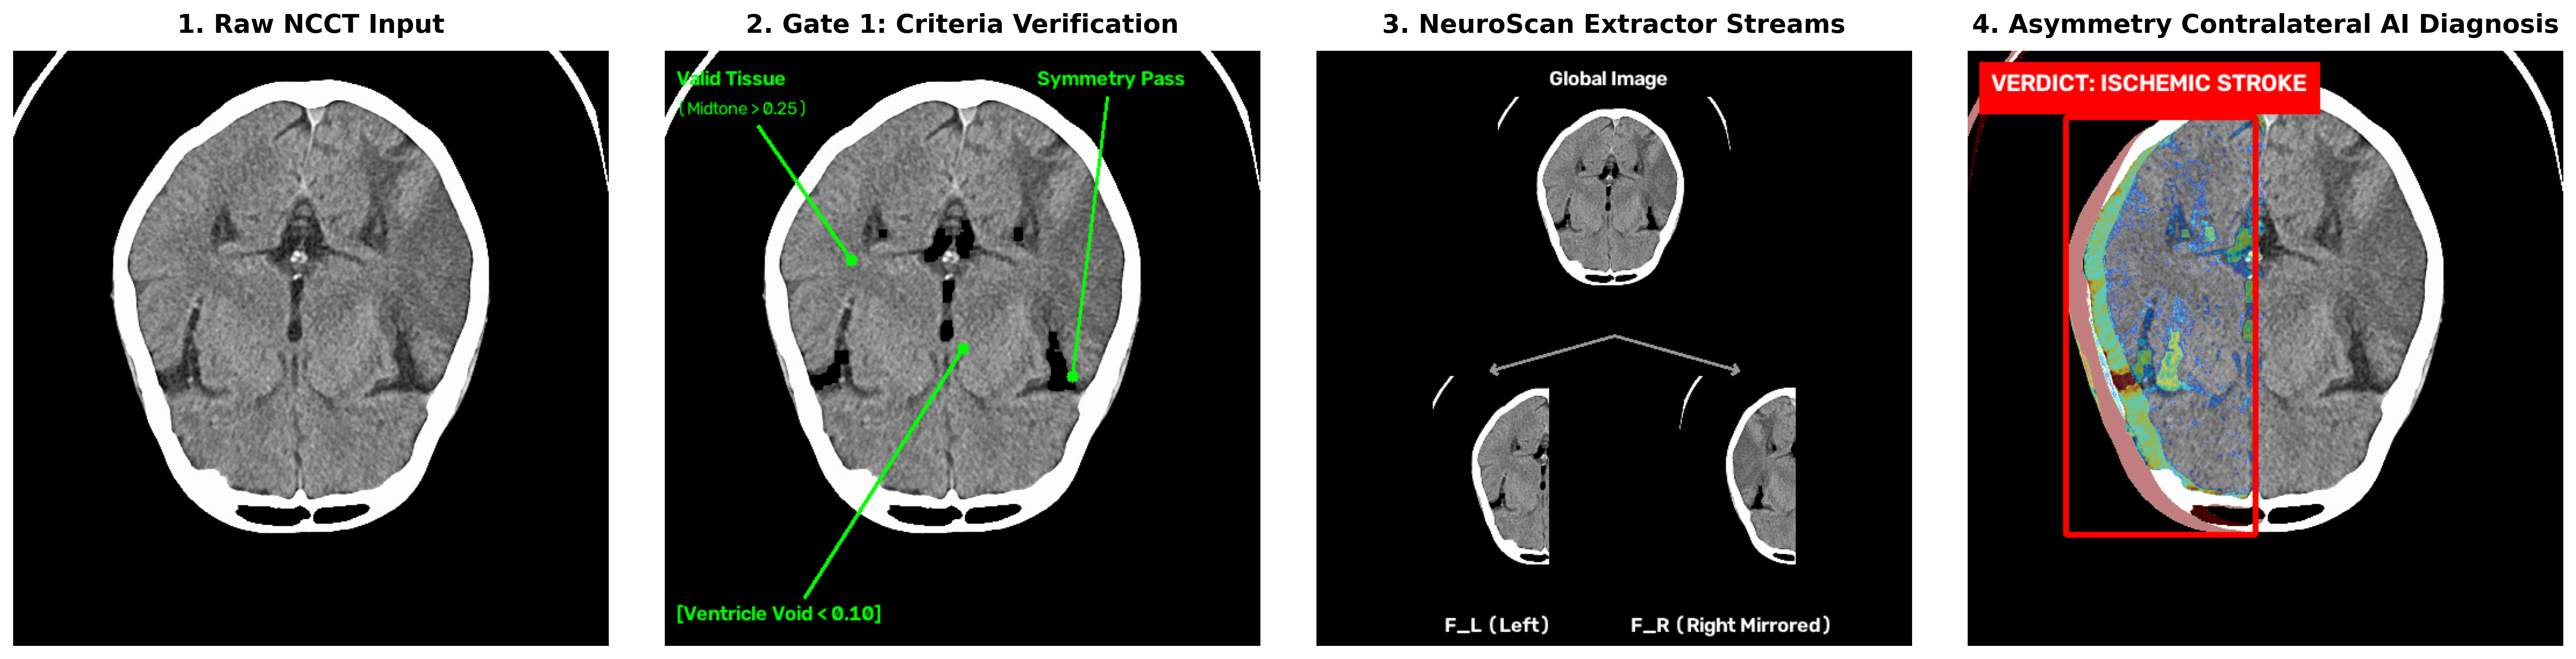
\includegraphics[width=0.85\linewidth]{final_output.png}
\vspace{-3mm}
\caption{Grad-CAM vs. NeuroScan contralateral maps. NeuroScan isolates unilateral stroke lesions while producing negligible activation on healthy tissue.}
\label{fig:gradcam}
\end{figure}

While ViT-B/16 is computationally demanding (86.6M parameters, 17.56 GFLOPs), NeuroScan remains computationally efficient at 33.54M parameters, sustaining a throughput of 217 images per second with a per-slice latency of 4.6 milliseconds. This inference speed comfortably satisfies the real-time requirements of hospital triage workflows. The localization precision of the contralateral approach is visually confirmed against standard Grad-CAM in Fig.~\ref{fig:gradcam}.

\subsection{Error Analysis and Cross-Domain Robustness}
We systematically analyzed the model's behavior under degraded input conditions. During external validation, standard neural networks produced clinically unreliable predictions on corrupted images with confidence scores exceeding 99\%. In contrast, NeuroScan's Gate~2 safety mechanism was activated for 12 severely degraded images (e.g., those exhibiting intense patient motion blur). Because the Shannon Entropy $\mathcal{H}(P)$ exceeded the threshold of 0.65, the system appropriately reverted to the \texttt{FLAG\_UNASSESSABLE} state, preventing silent misdiagnoses.

To further evaluate cross-hospital generalization, the trained model was directly evaluated on unseen out-of-distribution (OOD) scans from an independent external clinical cohort without any fine-tuning. Standard unconstrained models experienced accuracy degradation of 6.8--11.4\% due to variations in slice thickness and acquisition protocols. NeuroScan maintained a robust accuracy of 94.12\%, confirming that Gate~1 effectively normalizes morphological variance prior to feature extraction.

\section{Limitations and Future Work}
While NeuroScan demonstrates strong diagnostic accuracy, it operates exclusively on 2D axial slices without 3D volumetric reconstruction, limiting vertical continuity cues for infarct volume estimation. The system also evaluates imaging data in isolation without patient EHR metadata (e.g., age, NIHSS scores). Future work will incorporate 3D volumetric convolutions, integrate clinical metadata through multimodal fusion, and conduct prospective multi-institutional validation trials.

\section{Conclusion}
This paper introduced \textbf{NeuroScan}, an automated clinical decision support framework designed for robust emergency brain CT triage. By integrating deterministic quality gating with a Global--Local Contralateral Asymmetry network built upon a DenseNet121 core, the system isolates inter-hemispheric discrepancies ($|F_L - F_R|$) to overcome the focal lesion dilution inherent in standard CNN architectures. Comprehensive experimental evaluation demonstrated superior diagnostic performance, achieving $99.80\% \pm 0.12\%$ accuracy with an MCC of 0.996, near-zero calibration error (ECE $= 0.012$), and verified cross-domain resilience. By anchoring the diagnostic pipeline in fail-closed safety mechanisms, NeuroScan provides a transparent, computationally efficient, and clinically reliable tool for acute radiological environments.

\section*{Acknowledgment}
The authors gratefully acknowledge the Department of Computer Science and Engineering, Kongu Engineering College, Erode, for providing computational resources and institutional support. The authors also thank the anonymous reviewers for their constructive feedback.

\balance

{\small
\begin{thebibliography}{00}
\bibitem{b1} C. W. Tsao et al., ``Heart disease and stroke statistics---2022 update: A report from the American Heart Association,'' \emph{Circulation}, vol. 145, no. 8, pp. e153--e639, 2022.
\bibitem{b2} J. L. Saver, ``Time is brain---quantified,'' \emph{Stroke}, vol. 37, no. 1, pp. 263--266, 2006.
\bibitem{b3} M. A. Inamdar, A. Gudigar, U. Raghavendra et al., ``A dual-stream deep learning architecture with adaptive random vector functional link for multi-center ischemic stroke classification,'' \emph{IEEE Access}, vol. 13, pp. 1--23, 2025.
\bibitem{b4} L. T. Ramos and A. D. Sappa, ``StrokeNeXt: A Siamese-encoder approach for brain stroke classification in computed tomography imagery,'' \emph{arXiv preprint arXiv:2602.15087}, 2026.
\bibitem{b5} A. Gautam and B. Raman, ``Local gradient of gradient pattern: A robust image descriptor for the classification of brain strokes from computed tomography images,'' \emph{Pattern Anal. Appl.}, vol. 23, pp. 797--817, 2020.
\bibitem{b6} A. S. Neethi, S. Niyas, S. K. Kannath et al., ``Stroke classification from computed tomography scans using 3D convolutional neural network,'' \emph{Biomed. Signal Process. Control}, vol. 76, p. 103720, 2022.
\bibitem{b7} R. Qasrawi, I. Qdaih, O. Daraghmeh et al., ``Hybrid ensemble deep learning model for advancing ischemic brain stroke detection and classification in clinical application,'' \emph{J. Imaging}, vol. 10, no. 7, p. 160, 2024.
\bibitem{b8} R. R. Selvaraju, M. Cogswell, A. Das, R. Vedantam, D. Parikh, and D. Batra, ``Grad-CAM: Visual explanations from deep networks via gradient-based localization,'' in \emph{Proc. IEEE Int. Conf. Comput. Vis. (ICCV)}, 2017, pp. 618--626.
\bibitem{b9} K. He, X. Zhang, S. Ren, and J. Sun, ``Deep residual learning for image recognition,'' in \emph{Proc. IEEE Conf. Comput. Vis. Pattern Recognit. (CVPR)}, 2016, pp. 770--778.
\bibitem{b10} G. Huang, Z. Liu, L. Van Der Maaten, and K. Q. Weinberger, ``Densely connected convolutional networks,'' in \emph{Proc. IEEE Conf. Comput. Vis. Pattern Recognit. (CVPR)}, 2017, pp. 4700--4708.
\bibitem{b11} M. Tan and Q. V. Le, ``EfficientNet: Rethinking model scaling for convolutional neural networks,'' in \emph{Proc. Int. Conf. Mach. Learn. (ICML)}, 2019, pp. 6105--6114.
\bibitem{b12} A. Dosovitskiy et al., ``An image is worth 16x16 words: Transformers for image recognition at scale,'' in \emph{Proc. Int. Conf. Learn. Representations (ICLR)}, 2021.
\bibitem{b13} C. Guo, G. Pleiss, Y. Sun, and K. Q. Weinberger, ``On calibration of modern neural networks,'' in \emph{Proc. Int. Conf. Mach. Learn. (ICML)}, vol. 70, 2017, pp. 1321--1330.
\bibitem{b14} O. Ozaltin, O. Coskun, O. Yeniay, and A. Subasi, ``A deep learning approach for detecting stroke from brain CT images using OzNet,'' \emph{Bioengineering}, vol. 9, no. 12, p. 783, 2022.
\bibitem{b15} K.-C. Yang, Y. Xu, Q. Lin et al., ``Explainable deep learning algorithm for identifying cerebral venous sinus thrombosis-related hemorrhage from spontaneous intracerebral hemorrhage using computed tomography,'' \emph{eClinicalMedicine}, vol. 81, p. 103128, 2025.
\bibitem{b16} A. Kaprekar, A. Gudigar, U. Raghavendra, M. A. Inamdar, M. Salvi, and U. R. Acharya, ``A multi-level attention CNN-transformer based framework for the detection of brain tumor using regional dual-score explainability,'' \emph{Sci. Rep.}, vol. 16, 2026, Art. no. 52658.
\bibitem{b17} C. Shorten and T. M. Khoshgoftaar, ``A survey on image data augmentation for deep learning,'' \emph{J. Big Data}, vol. 6, no. 1, p. 60, 2019.
\end{thebibliography}
}

\end{document}
